\chapter{Results}\label{ch:results}

In this chapter we want to describe the features of the software environment which are used for mobile thermal mapping solutions in the context of universities.

\begin{wrapfigure}[24]{I}{0.45\textwidth}
    \centering
    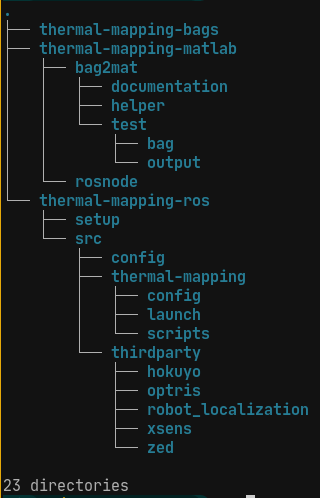
\includegraphics[width=0.35\textwidth]{img/results/folder_structure.png}
    \caption{The folder structure with different repositories for the thirdparty sensor nodes, bags, MATLAB application and the thermal-mapping node. The sensor nodes are sub repositories in the main ROS repository and the thermal-mapping node holds configs, scripts and the launch files.}
    \label{fig:folder_structure}
\end{wrapfigure}

\section{Data Acquisition}\label{ch:results:sec:dataAcquisition}

As described in section~\ref{ch:realization:sec:dataAcquisition} the different nodes and parts are stored in separated repositories.
This results in a folder structure with three directories for the bag, MATLAB and ROS part with the sensor repositories as sub repositories in the \texttt{thridparty} folder.
The structure with sub repositories guarantees that the nodes are compiled together with the \texttt{thermal-mapping} node and that they can be launched from one launch file.
As seen in figure~\ref{fig:folder_structure} the ROS repository also holds configurations, scripts to install the sensor drivers and the thermal-mapping node with different launch files.

There are three launch files:

\begin{enumerate}
    \item thermal\_mapping.launch
    \item thermal\_mapping\_display.launch
    \item thermal\_mapping\_reprocessing.launch
\end{enumerate}

The first starts only the sensor nodes which results in the node/topic graph in figure~\ref{fig:rosgraph_tf}.
The graph shows the relationships between nodes and topics where it gets clear that not all nodes are connected with each other.
That changes when the second launch file is used.
The seconds launch file invokes the first launch file and starts a \texttt{RVIZ} instance with a configuration to show the relevant data.
And the third launch file is for the case of reprocessing recorded data from a bag file.

\begin{figure}[h]
    \centering
    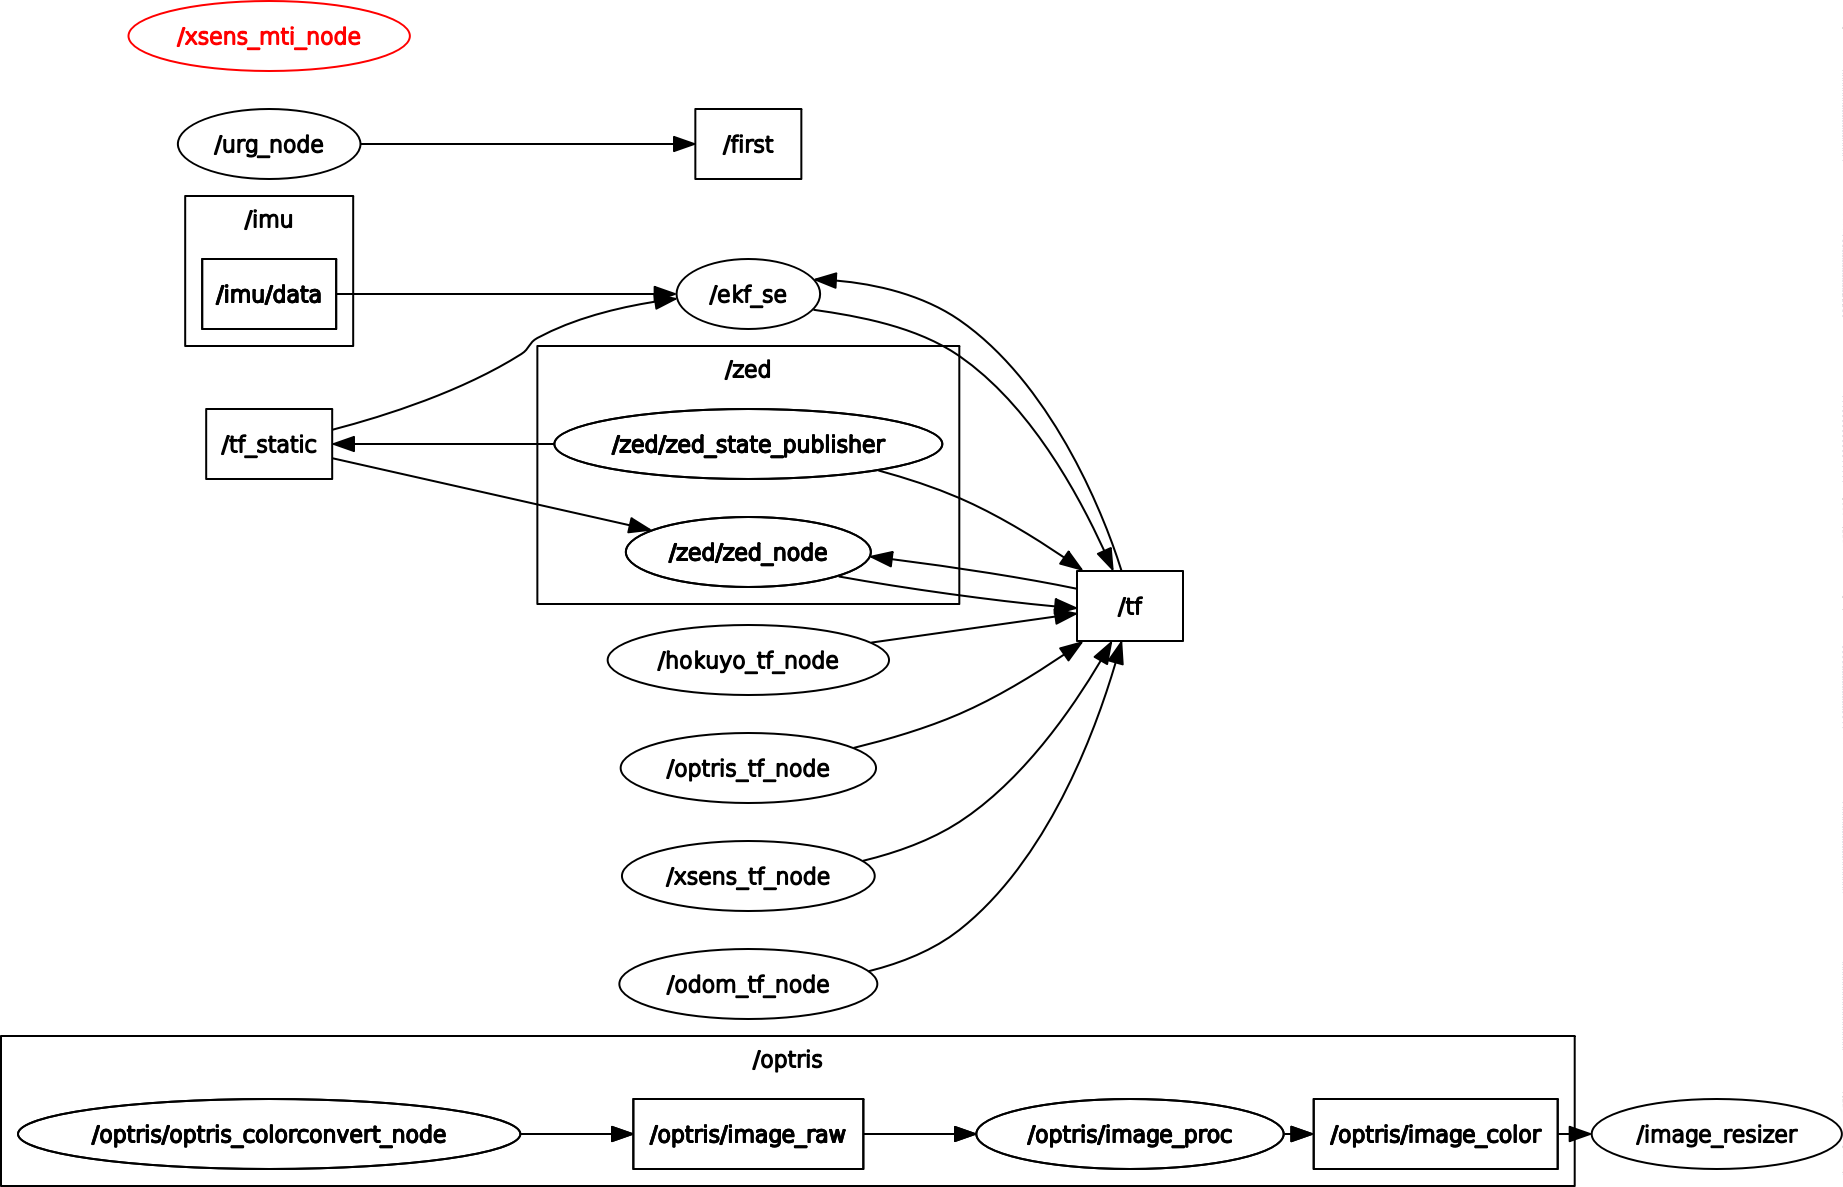
\includegraphics[width=\textwidth]{img/results/rosgraph_nodes_tf.png}
    \caption{The graph, generated with \texttt{RQT}, shows the different ROS nodes as elliptical shapes and the topics in rectangular shapes. Beside of this different name spaces are marked with a rectangle around the topics and nodes. The arrows between nodes and topics mark the relationship between them. An arrow to the topic indicates that the node publishes into the topic and an arrow pointing to a node indicates that the node subscribes to the topic.}
    \label{fig:rosgraph_tf}
\end{figure}

\begin{wrapfigure}[11]{I}{0.4\textwidth}
    \centering
    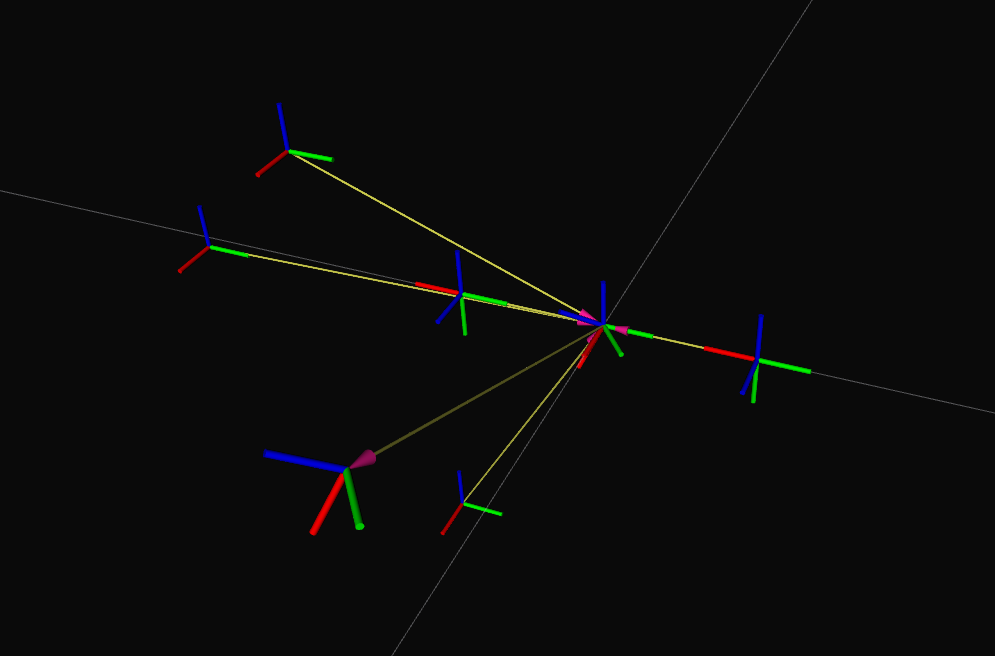
\includegraphics[width=0.3\textwidth]{img/results/tf_in_rviz.png}
    \caption{The different transformation and their relationships visualized in \texttt{RVIZ}.}
    \label{fig:tf_in_rviz}
\end{wrapfigure}

The visualization, started with the second or third launch file, depends on the tf-tree which can be seen in figure~\ref{fig:tf_tree}.
It also shows which node publishes the transformation and other information about average rate or buffer length.
But the main information from the tree is the topology of the different frames.
These frames are also visualized in \texttt{RVIZ} (figure \ref{fig:tf_in_rviz}) along with the other data.
In \texttt{RVIZ} it is also visualized which frames are connected per transformation but also how they are related to each other.

\begin{figure}[!ht]
    \centering
    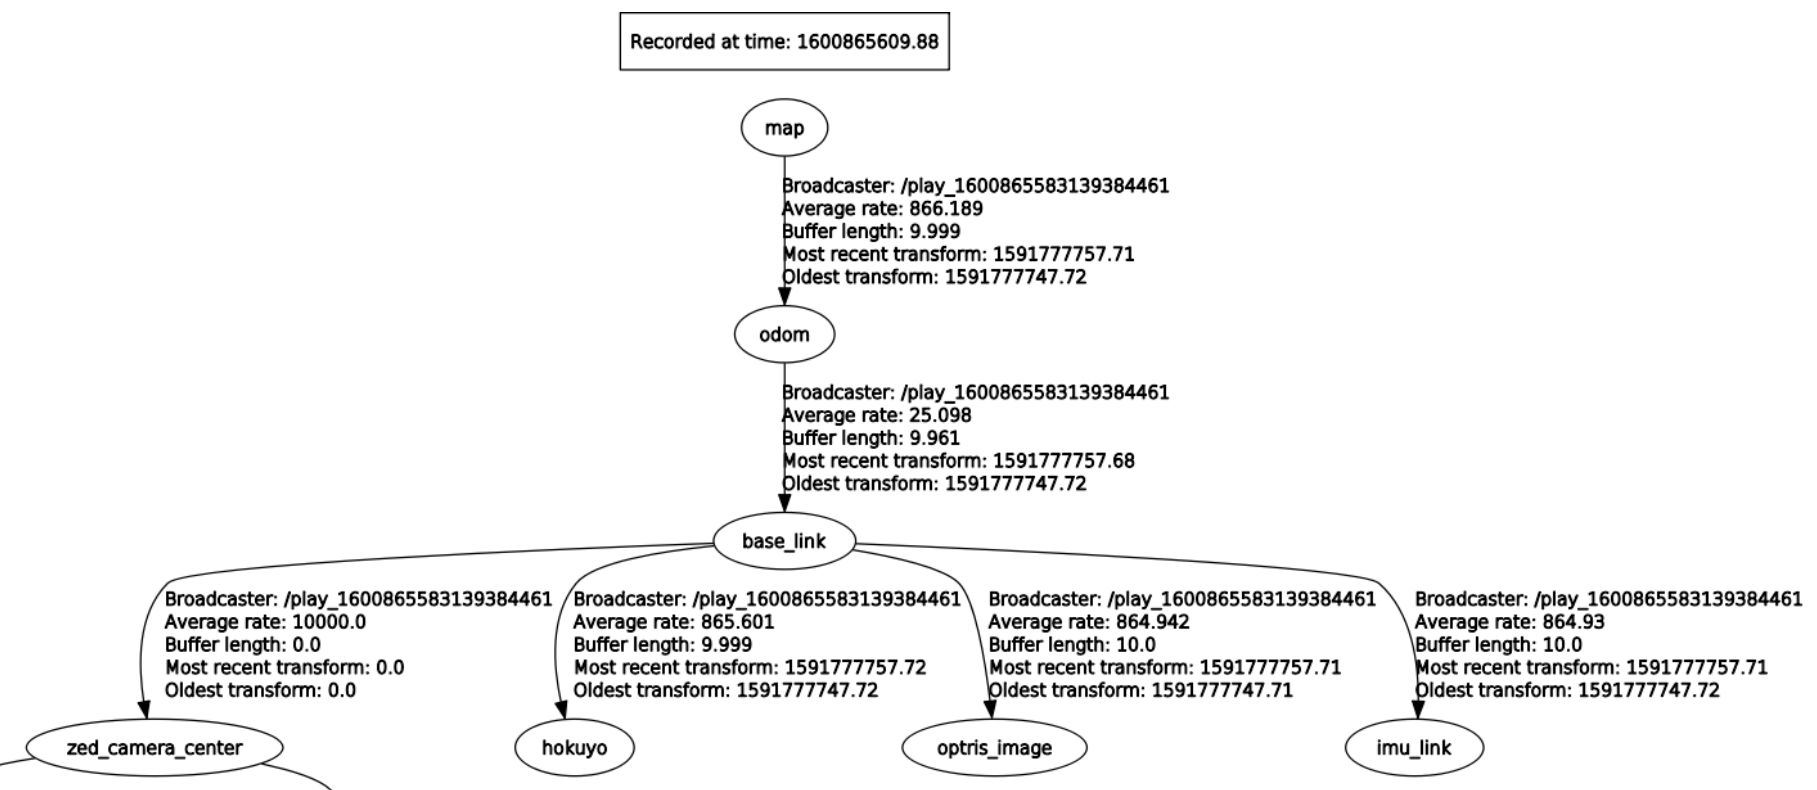
\includegraphics[width=\textwidth]{img/results/tf-tree.png}
    \caption{The tf-tree is visualized with \texttt{RQT} and shows which frame is the child of another frame. The transformation in this screenshot are all published by a rosbag play node. Due the restrictions because of covid19 we are forced to use a screenshot which is captured during a playback. The \texttt{zed\_camera\_center} is also the parent of other frames e.g.~the single lenses.}
    \label{fig:tf_tree}
\end{figure}

The 2.5D death image is visualized as a point cloud which is colorized with the framed thermal image.
But the thermal image doesn't fit perfectly to the shapes of the point cloud.

\begin{wrapfigure}[17]{I}{0.5\textwidth}
    \centering
    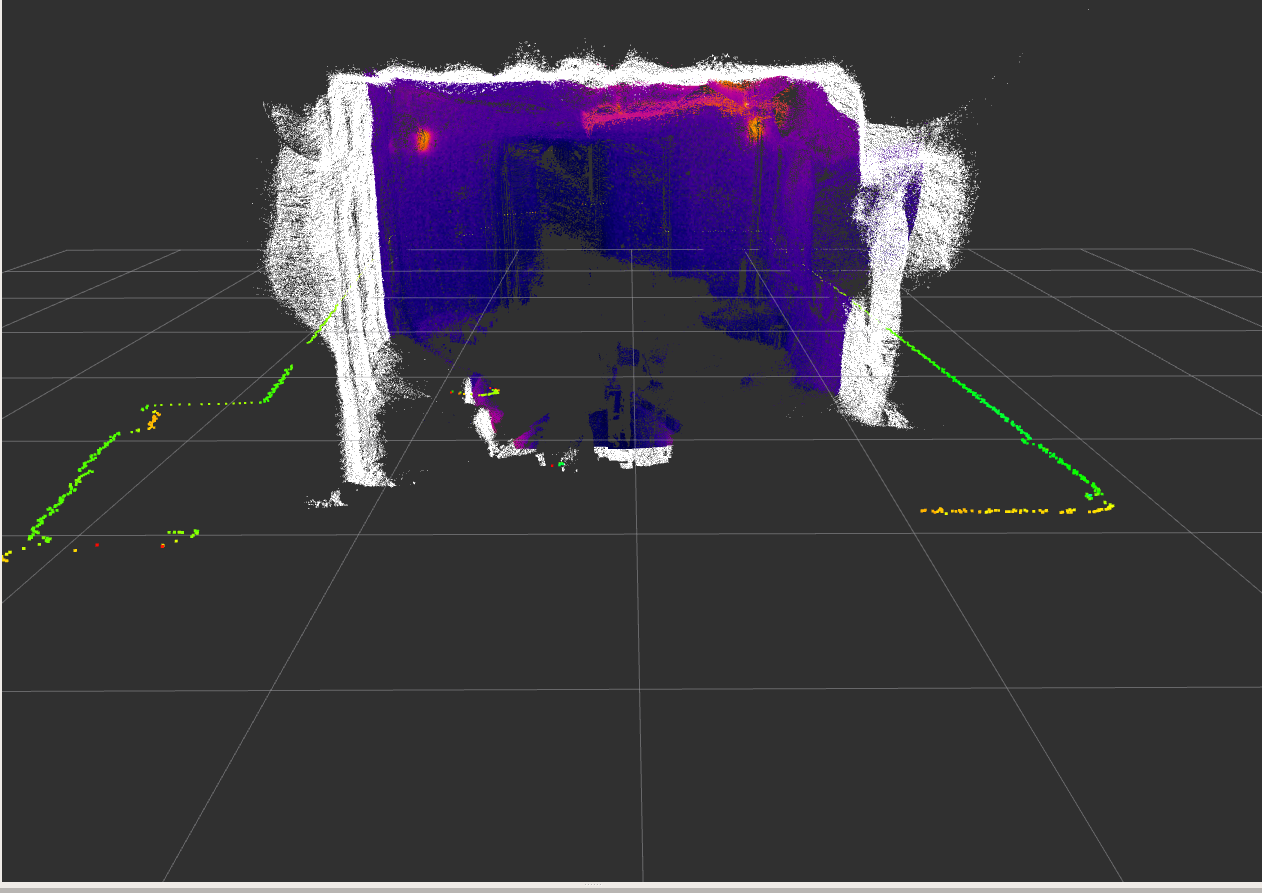
\includegraphics[width=0.5\textwidth]{img/results/rviz.png}
    \caption{The point cloud from the stereo camera colored with the frames image from the thermal camera and the measurements from the Lidar are visualized in RVIZ.}
    \label{fig:rviz}
\end{wrapfigure}

Lidar data are visualized as a line of points which roughly fit with the point cloud.
In figure~\ref{fig:rviz} it can be seen how the image data from the thermal camera, stereo camera and Lidar are visualized together.
The color of Lidar the lidar data is determined through the intensity reported by the sensor so that measurements from a window on the right side are colored in orange and solid walls are green.

While these data are easy to visualize the data from the IMU is only visualized by the transformation calculated by the extended kalmanfilter.
This takes effect when frame \texttt{map} is selected as base frame for the visualization.

Beside of the visualization the published data can also be saved as \texttt{*.bag} files by invoking the recording script inside the bag repository.
This script splits the files in 2GB big files and saves them inside the folder from where the script is invoked.

\section{Data Reprocessing}\label{ch:results:sec:dataReprocessing}

Reprocessing measurements is possible by using the recorded \texttt{*.bag} files.
These bag files can either be played with the rosbag tool or analysed with the MATLAB app.
While the bag is played the data can used with a node either written in C++, Python or MATLAB with the ROS-Toolbox.

\begin{wrapfigure}[29]{I}{0.7\textwidth}
    \centering
    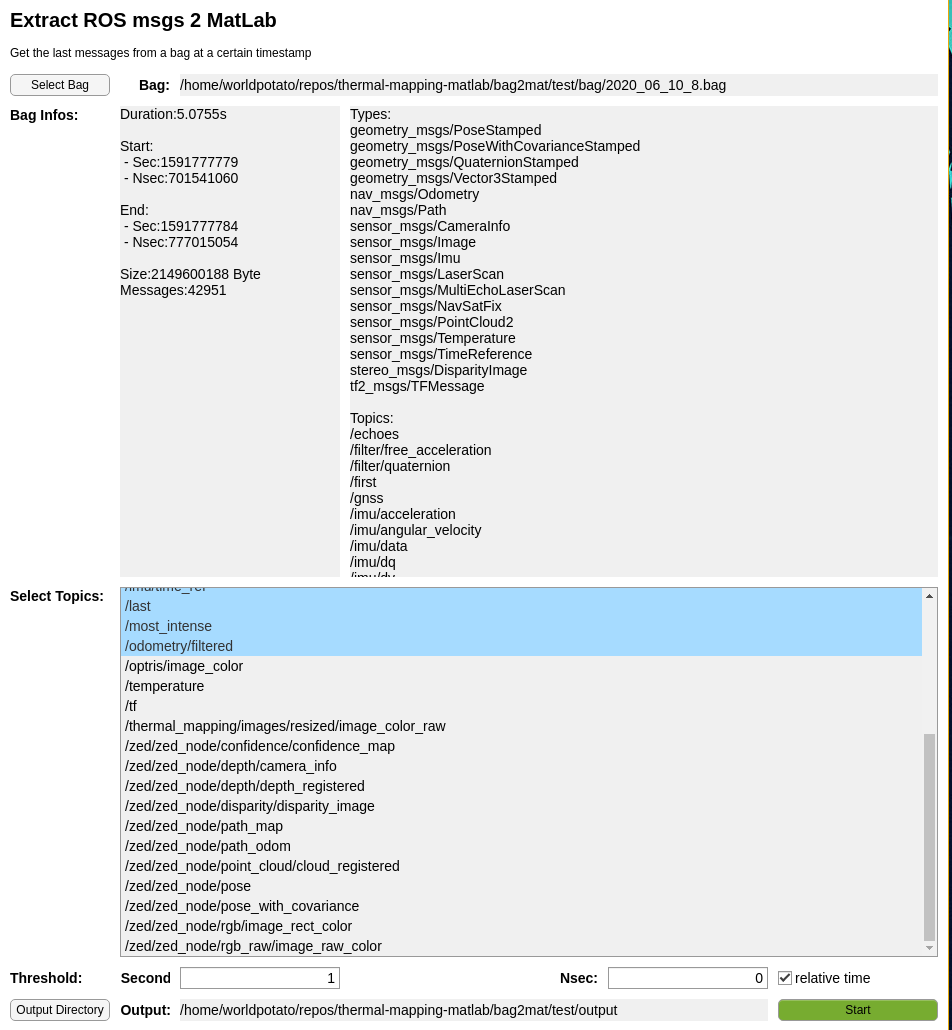
\includegraphics[width=0.7\textwidth]{img/results/matlab_app.png}
    \caption{The MATLAB app user interface to select the topics and a threshold time to extract single messages from bag files}
    \label{fig:matlab_app}
\end{wrapfigure}

But it's also possible to extract single data points with the MATLAB app.
The MATLAB application provides a graphical user interface to extract single messages as \texttt{*.mat} files.
As in figure~\ref{fig:matlab_app} the interface provides the list of available topics in the selected bag file.
The threshold time can be defined as absolute time or as relative time with respect to the start of the message.
After pressing the start button the last message publish before the threshold time in the selected topics will be extracted.
Together with the threshold time which defines the last possible timestamp from the extracted messages.

Both, the wrapper method and the MATLAB node, can be used to visualize the data inside the messages.
Examples how to archive the visualization are provides in the MATLAB repository.
A example of the visualization is shown in figure \ref{fig:matlab_visualization}.

\begin{figure}[b]
    \centering
    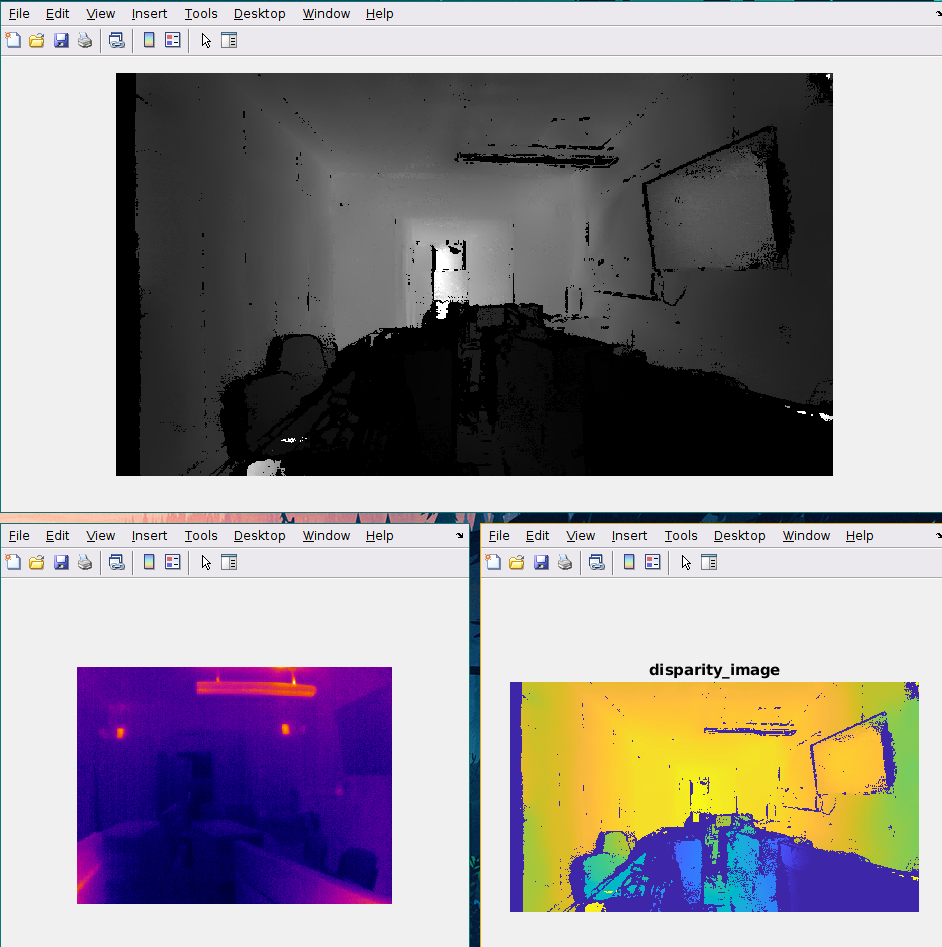
\includegraphics[width=\textwidth]{img/results/maltab_visualization.png}
    \caption{The visualization of the depth image, disparit image and the thermal image which is generated by MATLAB using the method to extract single messages with the ROS toolbox}
    \label{fig:matlab_visualization}
\end{figure}



